\title[Lecture slide retrieval]{Slide retrieval based on lecture recordings}
\author[V.\,Novotný]{Vít Novotný, witiko@mail.muni.cz}
\institute[FI MU]{Faculty of Informatics, Masaryk University}
\date{\today}
\subject{Project report}
\keywords{information retrieval, image processing, pattern recognition}

\maketitle

\begin{frame}
\frametitle<presentation>{Table of Contents}
\tableofcontents
\end{frame}

\section{Introduction}
Since the spring of 2004, the Faculty of Informatics at the Masaryk University
in Brno, Czech Republic (FI MU) has been recording lectures that take place in
the \abbr{D1}, \abbr{D2}, and \abbr{D3} lecture halls and making these
recordings available to students at the
\href{https://www.video.muni.cz}{video.muni.cz} web site as \term{digital video
files}~\cite{hladkaliska03lectures}. These recordings are a valuable learning
resource; however, due to the lack of information about the structure and the
content of these recordings, it is difficult to
\begin{enumerate}
\item retrieve recordings relevant to the user's \term{information need},
\item find relevant portions in the retrieved recordings, and
\item transform the information contained in the recording to a form that is more
  accessible to visually impaired users.
\end{enumerate}
As a result, the usefulness of these recordings is rarely fully exploited.

Most lecturers accompany their lectures with \term{lecture slides} that are shown
on the recordings and, at the same time, available for the students as a part of
the course materials in the form of structured \abbr{PDF} documents. One way to
add structured information to the recordings is then to find a mapping between the
temporal dimension of a recording and the pages of the corresponding lecture
slides. This gives us the digital form of the text that is being shown on any
given \term{frame} of the recordings, which can be immediately used to
\begin{enumerate}
\item retrieve portions of recordings relevant to the user's information need
  expressed in the form of a text query and
\item convey the text to the visually impaired user using a screen reader, a
  braille display, or another reading device.
\end{enumerate}
Other uses include the improvement of the perceived recording quality by
superimposing a high-resolution rendering of the \abbr{PDF} document pages on
the low-resolution digital video files.

The text is structured as follows: In Section~\ref{sec:problem}, I will
break down the problem into individual tasks and describe the evaluation
measures. In Section~\ref{sec:dataset}, I will describe the dataset
that I built for training, model selection, and performance evaluation.
In Section …

\section{Problem statement}
\label{sec:problem}
In this section, I will describe the problems associated with mapping lecture
recordings to lecture slide pages and I will specify the tasks a system will
need to solve.

\subsection{Sources of noise}
\label{sec:noise}
To better understand the intricacies of our task, let us first discuss what
kinds of \term{noise} we can expect to appear in our recordings.

\paragraph{Projection} Often, a lecturer will use an unpublished version of the
lecture slides that contains additional pages with \term{incrementally uncovered}
content. In this case, the lecture slides from the course materials may be a
poor match to what is shown on the recordings.

Occasionally, a lecturer will also show their lecture slides in a window rather
than in a full-screen mode. Therefore, finding the position of a projection
screen and finding the position of a lecture slide page within a
\term{projection screen} become two distinct tasks.

\paragraph{Scene} Due to the defects in the optical system of any camera, a
lecture room recording will suffer from a number of \term{aberrations} such as
defocus and distortion. In addition, if the camera is not perpendicular to a
projection screen, an \term{inverse perspective transform} of the recording
will be necessary to make the region corresponding to a projection screen
rectangular.

Let $\mathcal X$ be the \term{color space} of the lecture slides, $\mathcal Y$
the color space of the \term{projector}, and $\Phi_{\mathcal X},\Phi_{\mathcal
Y}$ the maps to the common color space $\mathbb K$. If the overlap between
$\Phi_{\mathcal X}(\mathcal X)$ and $\Phi_{\mathcal Y}(\mathcal Y)$ is small,
$\Phi^{-1}_{\mathcal Y}(\Phi_{\mathcal X}(\mathcal X))$ will be a poor
representation of $\mathcal X$. Even if $\Phi_{\mathcal X}(\mathcal
X)\approx\Phi_{\mathcal Y}(\mathcal Y)$, the \term{reflectance} of the
projection screen surface will distort the colors.

Due to the lightning conditions, the projection screen will in general be
\term{unevenly lit}.

\term{Obstacles} positioned between the \term{camera lens} and a projection
screen may partially obscure the recorded lecture slides.

\paragraph{Capture} The guesswork in assessing the \term{color temperature},
the presence of light sources that produce different color spectra compared to
\term{blackbodies}, and the potentially small overlap between $\Phi_{\mathcal
Y}(\mathcal Y)$ and $\Phi_{\mathcal Z}(\mathcal Z)$, where $\mathcal Z$ is the
color space of the projector, will further distort the colors.

Unlike lecture slides, which are generally provided in the form of vector
\abbr{PDF} documents, the resulting digital video files are a result of
\begin{enumerate}
  \item temporal sampling into frames at a given \term{framerate},
  \item spatial sampling at a given \term{resolution},
  \item light frequency sampling at a given \term{color depth},
  \item \term{chroma subsampling}, and 5. \term{lossy compression}
\end{enumerate}
applied to the original recording. Each of the above reduces the amount of
information present in the digital video file.

\subsection{Tasks}
\label{sec:tasks}
Given the above analysis, a system mapping lecture recordings to lecture slides
will need to solve the following tasks listed in bottom-up order:
\begin{enumerate}
  \item assessing the similarity between a cropped-out projection screen and
    lecture slides, namely
    \begin{enumerate}
      \item mapping a cropped-out projection screen to a lecture slide page, and
      \item deciding if a projection screen matches any lecture slide page,
    \end{enumerate}
  \item detecting and cropping out all projection screens in a single frame
    of a recording, and
  \item selecting important frames and the order in which frames are resolved.
\end{enumerate}
I will now describe the individual tasks in detail along with the proposed
evaluation method.

\paragraph{Task 1a} Given a single cropped-out projection screen and a set of
lecture slide pages, the task is to retrieve the page in the set that is most
similar to the screen. Since a screen and the matching page may not be
perfectly aligned, rotation~\cite{smith1995simple}, and
translation~\cite{sarvaiyaetal09} coupled with scaling may be necessary to
\term{register} each screen-page tuple before the removal of the noise
described in Section~\ref{sec:noise}.

I will frame this task as an \term{information retrieval} (\abbr{IR}) problem,
i.e. we will be looking for an \abbr{IR} system that ranks pages by their
similarity to a screen and, if there exists a matching page, it will be placed
first. To compare two systems, we can estimate the expected value of the
\term{rank} of a matching page produced by each system across one or several
test dataset.

\paragraph{Task 1b} Given a single cropped-out projection screen and a set of
lecture slide pages, the task is to decide whether or not the screen matches
any page in the set.  If a task 1a system produces for each screen not only a
ranking of pages, but also an estimate of distance, similarity, match
confidence, or match probability for each page, and if the random vector of
these estimates can be expected to have a different probability distribution
in the positive case (when a screen matches) and in the negative case, then a
classifier can be trained on one or several training datasets using the
measures produced by a task 1a system as features.

If two systems only produce binary decisions, then we can estimate the expected
values of the \term{misclassification loss} to compare them. If two systems
also report the decision confidence expressed by the distance from a
\term{decision hyperplane}, then we can estimate the expected value of the
\term{binomial deviance}~\cite[sec.~10.6]{friedman2001elements} to compare the
systems. Alternatively, if two systems produce a posterior probability
estimate, then we can estimate the expected values of the
\term{log-likelihood}~\cite[sec.~2.6.3]{friedman2001elements} to compare the
systems.
Informally speaking, both binomial deviance and log-likelihood favor
classifiers that are hesitant about their wrong decisions and confident about
their correct decisions.

\paragraph{Task 2} Given a single recording frame, the task is to detect the
boundaries of all lit projection screens. To compare two systems, we can
estimate the expected value of the \term{Jaccard index} between each system and
one or several test datasets using polygonal union and intersection.

\paragraph{Task 3} Given a single recording, the task is to detect the frames
at which the following events take place:
\begin{enumerate}
  \item a new projection screen is lit,
  \item a projection screen is no longer lit, or
  \item a projection screen shows new content.
\end{enumerate}
To compare two systems, we can take events of each type and estimate the
expected value of standard segmentation similarity metrics such as boundary
similarity ($\textrm B$)~\cite{P13-1167} for the event type between each system
and one or several test datasets.

\section{Dataset}
\label{sec:dataset}
As a first step in building and evaluating a system solving the above tasks, I
built a dataset from the recordings published at \url{https://video.muni.cz}.
Although the recordings date as far back as 2004, I restricted myself to the
recordings from the \abbr{D1}, \abbr{D2}, and \abbr{D3} lecture halls taken
during 2010--2016. This was mainly due to the difficulty in reaching out to
the lecturers who are often no longer a part of the faculty, and the variance
in the video file format encoding and resolution. From the uniform distribution
of these recordings, I drew a random sample that would form my dataset.
The original sample consisted of 20 recordings. For three recordings, I was
unable to establish communication with the lecturers to request their consent.
For three other recordings, the lecturers would not give consent to including
the recordings in the dataset; I drew three recordings from the uniform
distribution of recordings as substitutes.

The dataset has been published in a Git repository at
\url{https://gitlab.fi.muni.cz/xnovot32/fi-muni-video-699}.
% TODO: Document the license, make the repository public (move the GitHub perhaps)?

\subsection{Dataset structure}
The dataset consists of 17 recordings. For the purpose of solving tasks 1 and
2, a recording consists of a set of lecture slides and a sample of the video
file frames. Since the systems solving tasks 1 and 2 will only be invoked by
the system solving task 3 when one of the events described in
Section~\ref{sec:tasks} takes place, I did not assume uniform distribution of
the frames when drawing a sample. Instead, I reduced each uneventful segment of
the recording into a single frame by drawing from the uniform distribution of
frames forming the segment. A random sample of up to 25 frames was then drawn
from the uniform distribution of the reduced segments. For each frame in the
sample, I marked the boundaries of all lit screens and described the pages of
the lecture slides shown on the screens.

The dataset is represented by an \abbr{XML} document \texttt{dataset.xml} in
the language \texttt{dataset.xsd} shown in Figure~\ref{fig:schema}. The root
element of \texttt{dataset.xml} consists of a sequence of recordings
represented by video elements. I will now describe the individual elements of
the language.

\begin{figure}
\leavevmode\kern-0.2\textwidth
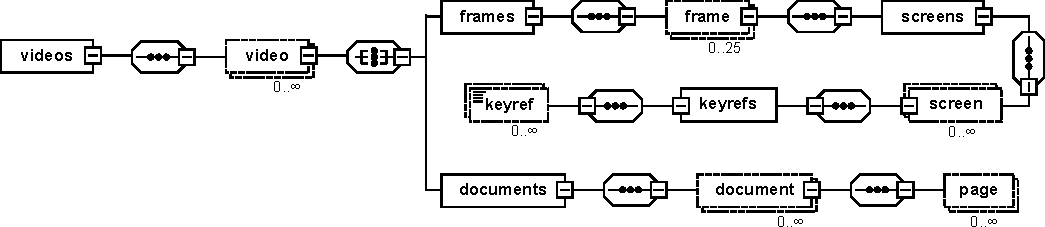
\includegraphics[width=1.4\textwidth]{fig/schema}
\caption{The \abbr{XML} language \texttt{dataset.xsd} \iffalse produced using the
  \term{\abbr{XSD} diagram} tool\fi}
\label{fig:schema}
\end{figure}

\afterpage{%
\begin{landscape}
\begin{figure}
\thisfloatpagestyle{empty}
\leavevmode\kern-.09\paperheight
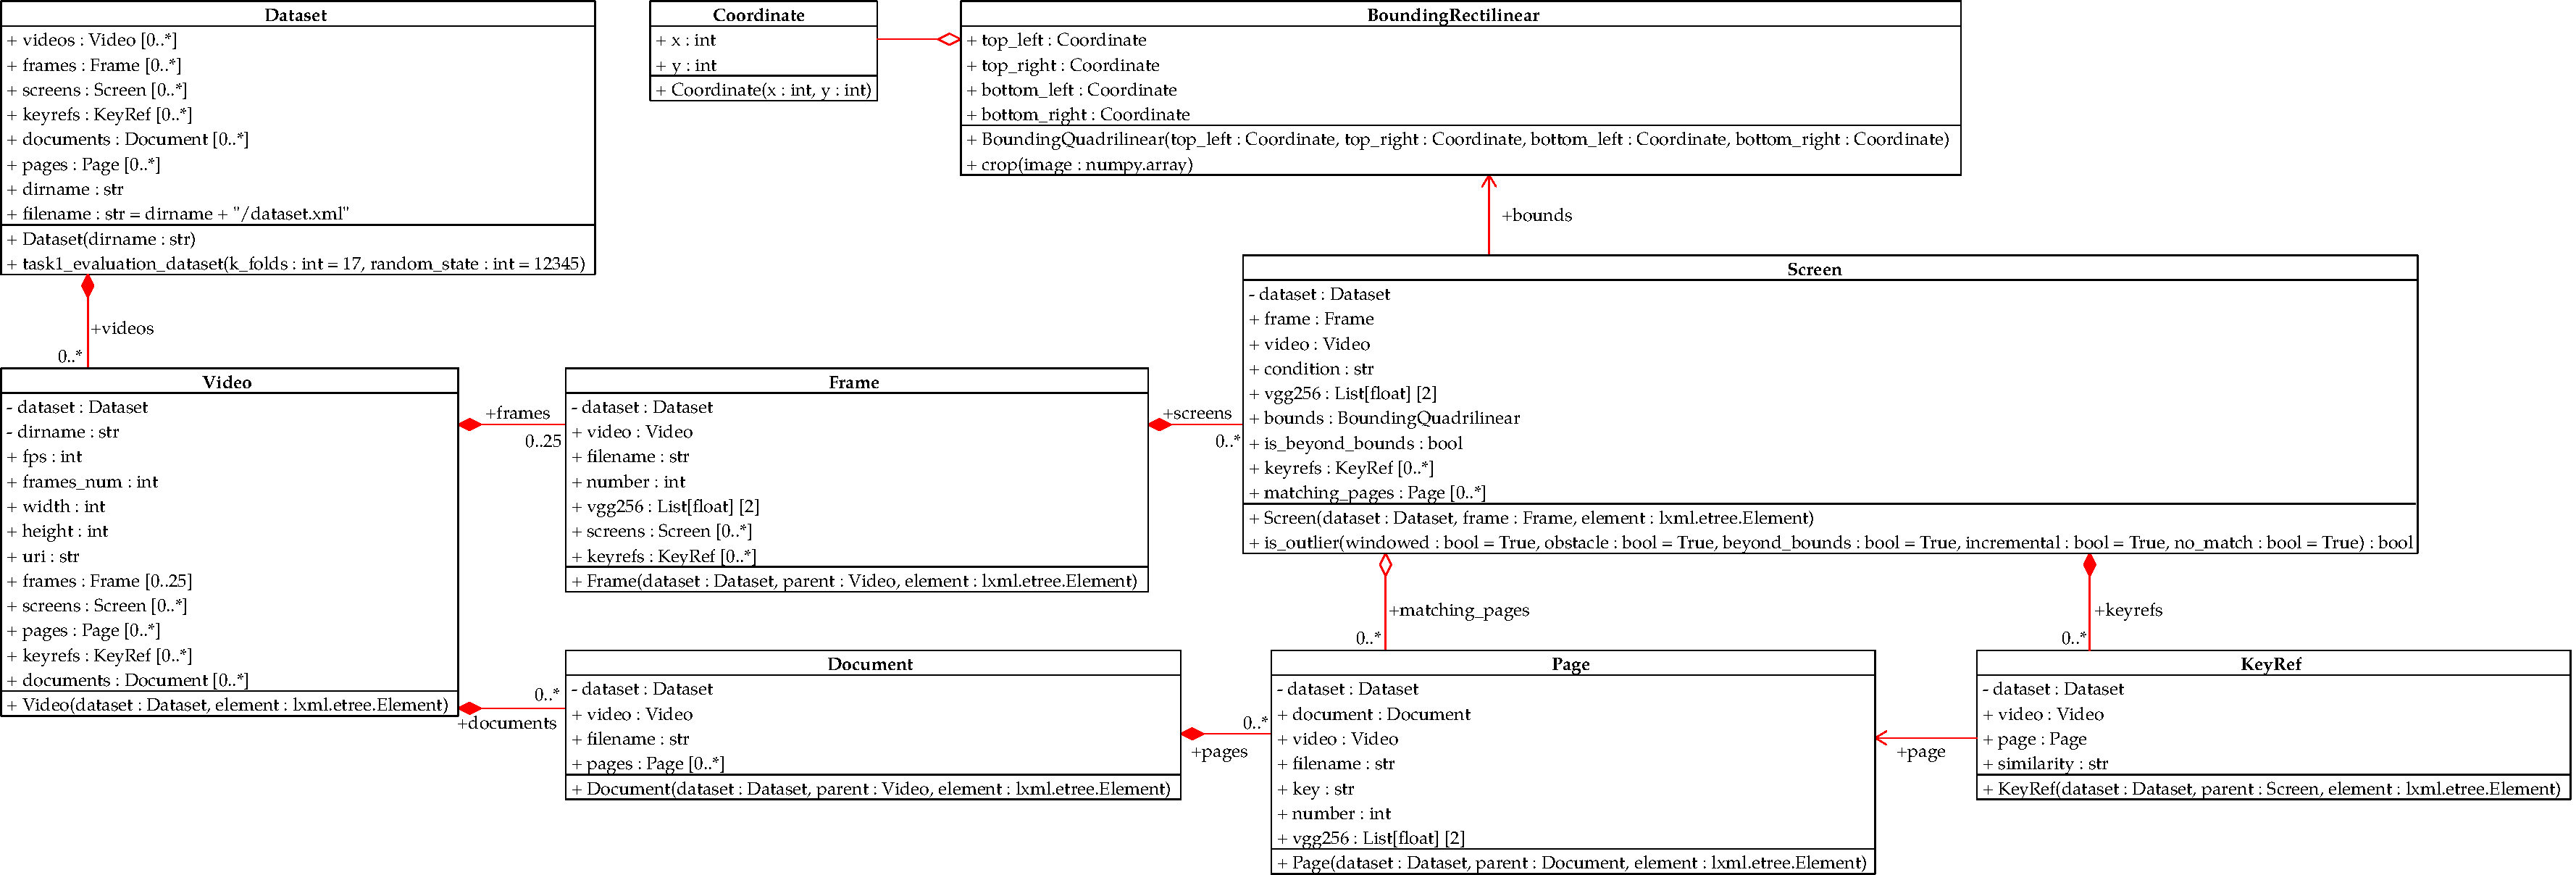
\includegraphics[width=.9\paperheight]{fig/uml}
\caption{A \abbr{UML} class diagram of the Python interface for the dataset
  \iffalse produced using the \term{Umbrello} tool\fi}
\label{fig:uml}
\end{figure}
\end{landscape}}

\subsubsection*{The video element}
A video element corresponds to a single lecture recording and contains the
following attributes:
\begin{description}
  \item[dirname] the name of the directory containing the frames and lecture slides,
  \item[uri] an \abbr{URI} of the video file containing the recording,
  \item[fps] the framerate of the video file,
  \item[frames] the length of the video file in frames, and
  \item[width\textmd, height] the resolution of the video file.
\end{description}
Beside the attributes, a video element contains a sequence of recording frames
and lecture slides represented by frame elements and document elements,
respectively.

\subsubsection*{The frame element}
A frame element corresponds to a single frame of a recording and contains the
following attributes:
\begin{description}
  \item[number] the frame number in the video file,
  \item[vgg256] two baseline feature vectors obtained by feeding the entire
    frame into 256dimensional \term{\abbr{VGG} convolutional neural
    networks}~\cite{simonyan2014very} and taking the state of the last hidden
    layer, and
  \item[filename] the filename of the image file containing the frame.
\end{description}
Beside the attributes, a frame element contains a sequence of lit projection
screens represented by screen elements.

\subsubsection*{The screen element}
A screen element corresponds to a single lit projection screen on a single
frame of a recording and contains the following attributes:
\begin{description}
  \item[x0\textmd, y0\textmd, x1\textmd, y1\textmd, x2\textmd, y2\textmd,
        x3\textmd, y3] coordinates with respect to the current frame
    of the recording that specify the four corners of a quadrilinear
    bounding a single lit projection screen,
  \item[condition] the types of noise affecting this frame of the recording:
    \begin{description}
      \item[windowed] the projection screen shows a lecture slide in a window
        rather than in a full-screen mode,
      \item[obstacle] an obstacle positioned between the camera lens and the
        projection screen partially obscures the lecture slide, and
      \item[pristine] none of the above, and
    \end{description}
  \item[vgg256] two baseline feature vectors obtained by feeding the
    cropped-out projection screen frame into 256dimensional \abbr{VGG}
    convolutional neural networks and taking the state of the last hidden
    layer.
\end{description}
Beside the attributes, a screen element is in a relation to pages of lecture
slides that is represented by a sequence of keyref elements.

\subsubsection*{The keyref element}
A keyref element corresponds to a single 2-tuple from a binary relation between
lit projection screens and lecture slide pages and contains the following
attribute:
\begin{description}
  \item[similarity] the type of relation between this lit projection screen and
    a lecture slide page:
    \begin{description}
      \item[full] the projection screen shows the entire lecture slide, and
      \item[incremental] the \term{logical page} shown in the projection screen
        is split to several \term{physical pages} in the lecture slides and
        incrementally uncovered.
    \end{description}
\end{description}
Beside the attribute, a keyref element contains a reference to a lecture slide
page represented the unique identifier of a page element.

\subsubsection*{The document element}
A document element corresponds to a single set of lecture slides and contains
the following attribute:
\begin{description}
  \item[filename] the filename of the \abbr{PDF} file containing the lecture slides.
\end{description}
Beside the attribute, a document element contains a sequence of lecture slide
pages screens represented by page elements.

\subsubsection*{The page element}
Each page element corresponds to a single page of lecture slides and contains
the following attribute:
\begin{description}
  \item[key] a identifier of the page that is unique in the current video element,
  \item[filename] the filename of the image file containing the page,
  \item[number] the number of the page in the \abbr{PDF} document,
  \item[vgg] two baseline feature vectors obtained by feeding the
    page into 256dimensional \abbr{VGG} convolutional neural networks and
    taking the state of the last hidden layer.
\end{description}

The dataset is distributed along with a Python interface implemented in files
\texttt{dataset.py} and \texttt{review.py} whose class diagram is shown in
Figure~\ref{fig:uml}.

\subsection{Examples}
To give a better sense of the structure and the content of the dataset, I will
now give several examples along with the corresponding \abbr{XML} code, and the
images of the recording frames, projection screens, and lecture side pages.

\begin{description}
  \begin{figure}
    \inputminted{xml}{fig/examples/normal/example.xml}
    \exampleimages{fig/examples/normal}%
      {frame006000.png}{frame006000-00.png}{slides01-30.png}
    \caption{A screen element in the usual case. Both the abbreviated code
      of the \texttt{dataset.xml} document (above) and the recording frame,
      cropped-out projection screen, and the lecture slide page (below) are
      shown.}
    \label{fig:example-normal}
  \end{figure}
  \item[The usual case] For 371 out of the total 683 screen elements, the
    projection screen is captured fully without any obstacles positioned
    between the camera lens and the screen and it shows a single page from the
    associated lecture slides in full-screen mode. An example is shown in
    Figure~\ref{fig:example-normal}.

  \begin{figure}
    {\renewcommand\fcolorbox[4][rgb]{#4\kern1pt}% Remove rectangles around bad syntax.
     \inputminted{xml}{fig/examples/obstacle/example.xml}}
    \exampleimages{fig/examples/obstacle}%
      {frame090000.png}{frame090000-01.png}{slides01-28.png}
    \caption{A screen element obscured by an obstacle positioned between the
      camera lens and the projection screen. Both the abbreviated code of the
      \texttt{dataset.xml} document (above) and the recording frame,
      cropped-out projection screen, and the lecture slide page (below) are
      shown.}
    \label{fig:example-obstacle}
  \end{figure}
  \item[Obscured projection screen] For 5 out of the total 683 screen elements,
    the projection screen is partially obscured by an obstacle positioned
    between the camera lens and the screen. An example is shown in
    Figure~\ref{fig:example-obstacle}
\end{description}

\section{System description}
\section{Experimental setup}
\section{Results}
\section{Conclusion}

\iffalse

\section[Short Section 1 Name]{Full Section 1 Name}
\subsection[Short Subsection 1 Name]{Full Subsection 1 Name}

\begin{frame}{Frame Title}{Frame Subtitle}
plain text, \structure{page structure}, \alert{emphasis}
\begin{itemize}
  \item a single-line bullet list item
  \item a bullet list item that is quite long (in order to force a line break),
    which also contains \alert{emphasized text}
  \begin{itemize}
    \item a second-level list item
    \begin{itemize}
      \item a third-level list item
    \end{itemize}
    \alert{\item an emphasized second-level list item}
  \end{itemize}
\end{itemize}
\begin{enumerate}
  \item a numbered list item
  \begin{enumerate}
    \item a second-level list item containing a math expression
      \[ E = mc^2 \]
  \end{enumerate}
\end{enumerate}
\end{frame}

\subsection[Short Subsection 2 Name]{Full Subsection 2 Name}

\begin{frame}{Text Blocks}
text above a block
\begin{block}{Block}
  text
\end{block}
\begin{exampleblock}{Example Block}
  text
\end{exampleblock}
\begin{alertblock}{Emphasized Block}
  text
\end{alertblock}
text below a block\footnote{a footnote with an \url{http://address.edu}}
\end{frame}

\begin{frame}{Figures}
\begin{figure}
  \includegraphics[width=.5\textwidth,height=.5\textheight,keepaspectratio]{cow-black.mps}
  \caption{A Holstein Friesian cow}
\end{figure}
\end{frame}

\subsection[Short Subsection 3 Name]{Full Subsection 3 Name}

\begin{frame}{Tables}
\begin{table}
  \begin{tabular}{llc}
    First Name & Surname & Year of Birth \\ \midrule
    Albert & Einstein & 1879 \\
    Marie & Curie & 1867 \\
    Thomas & Edison & 1847 \\
  \end{tabular}
  \caption{The great minds of the 19th century}
\end{table}
\end{frame}

\makeatletter
\begin{frame}{Automatic Optical Scaling}
\begin{center}
\begin{tabular}{ll}
\Huge \f@family & \Huge \structure{\f@size pt} \\
\huge \f@family & \huge \structure{\f@size pt}  \\
\LARGE \f@family & \LARGE \structure{\f@size pt}  \\
\Large \f@family & \Large \structure{\f@size pt}  \\
\large \f@family & \large \structure{\f@size pt}  \\
\normalsize \f@family & \normalsize \structure{\f@size pt}  \\[-0.95pt]
\small \f@family & \small \structure{\f@size pt}  \\[-1.95pt]
\footnotesize \f@family & \footnotesize \structure{\f@size pt} \\[-2.95pt]
\scriptsize \f@family & \scriptsize \structure{\f@size pt}  \\[-4.95pt]
\tiny \f@family & \tiny \structure{\f@size pt}
\end{tabular}
\end{center}
\end{frame}
\makeatother

\fi

\begin{frame}<presentation>[plain]
\vfill
\centerline{Thank you for your attention!}
\vfill\vfill
\end{frame}

\printbibliography
